%!TEX root = ../intro.tex
%******************************
%	 Biological noise 
%*****************************

\section{Biology of expression noise} 

Biological noise is defined as measurable differences in \gls{mRNA} or protein abundance across homogeneous cell populations (see \textbf{Box 1}). 
%Predominantly, scRNA-Seq technologies, single molecule fluorescence in situ hybridization (smFISH) or fluorescence reporter assays were used to measure the variation in mRNA or protein abundance. 
All cellular systems are exposed to varying levels of noise and employ strategies to make use of or cope with this source of variation. The sources and consequences of biological noise have been studied in an array of viral, prokaryotic and eukaryotic systems while its functional role is controversially discussed depending on the system \citep{Raj2010, Balazsi2011, Eldar2010}. It is crucial to differentiate between unicellular organisms (prokaryotes, viruses, and yeast) in which mainly positive effects of biological noise are described and higher, multicellular eukaryotic systems where biological noise either benefits or obstructs cellular function depending on the tissue type and health state.\\

\begin{Comment}
\textbf{Box 1: Defining biological noise}\\
\small
Biological noise in cell populations arises from stochastic effects on transcription and translation that propagates to form cell-to-cell phenotypic differences. To define noise, one needs to distinguish between different sources of cell-to-cell variability in multiple measurable factors. On the broadest level, differences between single cells in a population can arise from structured (also termed “deterministic” in Marusyk \emph{et al.}, 2012 \citep{Marusyk2012}) and unstructured sources (similar as in Singer \emph{et al.}, 2014 \citep{Singer2014}). When cell populations containing discrete cell-states and/or cell-types are captured \citep{Paul2015, Ibarra-Soria2018, Rosenberg2018}, measuring cell-specific features results in the detection of non-stochastic but rather correlated (structured) differences between individual cells. In cell populations where correlated features do not allow the detection of groups (unstructured variation), continuous processes (e.g.~differentiation) can be the dominating source of cell-to-cell phenotypic variability \citep{Dahlin2018}. Computational approaches allow the detection of these trajectories (e.g.~via principal component analysis or pseudotime inference \citep{Trapnell2014, Angerer2015}). Here, I therefore define biological noise as unstructured, phenotypic cell-to-cell differences independent of measurement errors. 
As previously introduced \citep{Elowitz2002}, biological noise can broadly arise from intrinsic and extrinsic sources. Intrinsic noise originates from stochastic biochemical effects within one cell that directly influences gene-specific expression \citep{Swain2002} (e.g.~transcription factor binding dynamics). Extrinsic noise on the other hand introduces co-expression across multiple genes (also in a pathway specific manner \citep{Raser2010}) due to differences in cell-specific factors such as stress response, mitochondrial maintenance, amino-acid synthesis \citep{Stewart-Ornstein2012} or cell-cycle \citep{Zopf2013}. Intrinsic noise can therefore be measured as expression differences between co-regulated genes in one cell while extrinsic noise is measured as co-regulated variance in gene sets across all cells.\\
\end{Comment}

\subsection{Bet-hedging in unicellular systems}

Biological noise has been described to trigger the differential decision between latency and replication in viruses such as \Gls{HIV} and the \gls{lambdaPhage}. In the case of the \gls{lambdaPhage}, infected cells either reside in a lysogenic state where the genetic material of the virus is transmitted to daughter cells without inducing cell death or a lytic state where the virus destroys the host cell \citep{Lieb1953}. Previous studies have shown that the lysis-lysogeny switch in \gls{lambdaPhage} is driven by intrinsic and extrinsic noise \citep{Arkin1998, St-Pierre2008}. This idea has been extended by Zeng \textit{el al.}, 2010 where the lysis-lysogeny switch does not depend on a single noise-driven decision but on the sum of all individual phages per cell \citep{Zeng2010}. A similar ‘bet-hedging’ strategy, a probabilistic decision between multiple states, exists for \Gls{HIV} infection. Upon infection, \Gls{HIV} either rapidly replicates or resides in a long-lived latent state from which the virus can switch to replication \citep{Weinberger2015}. It has been shown that combining noise-enhancing and activating drugs shifts latent viruses into the active-replication state that can be targeted by anti-retroviral therapeutics \citep{Dar2014}. 

\begin{figure}[!h]
\centering
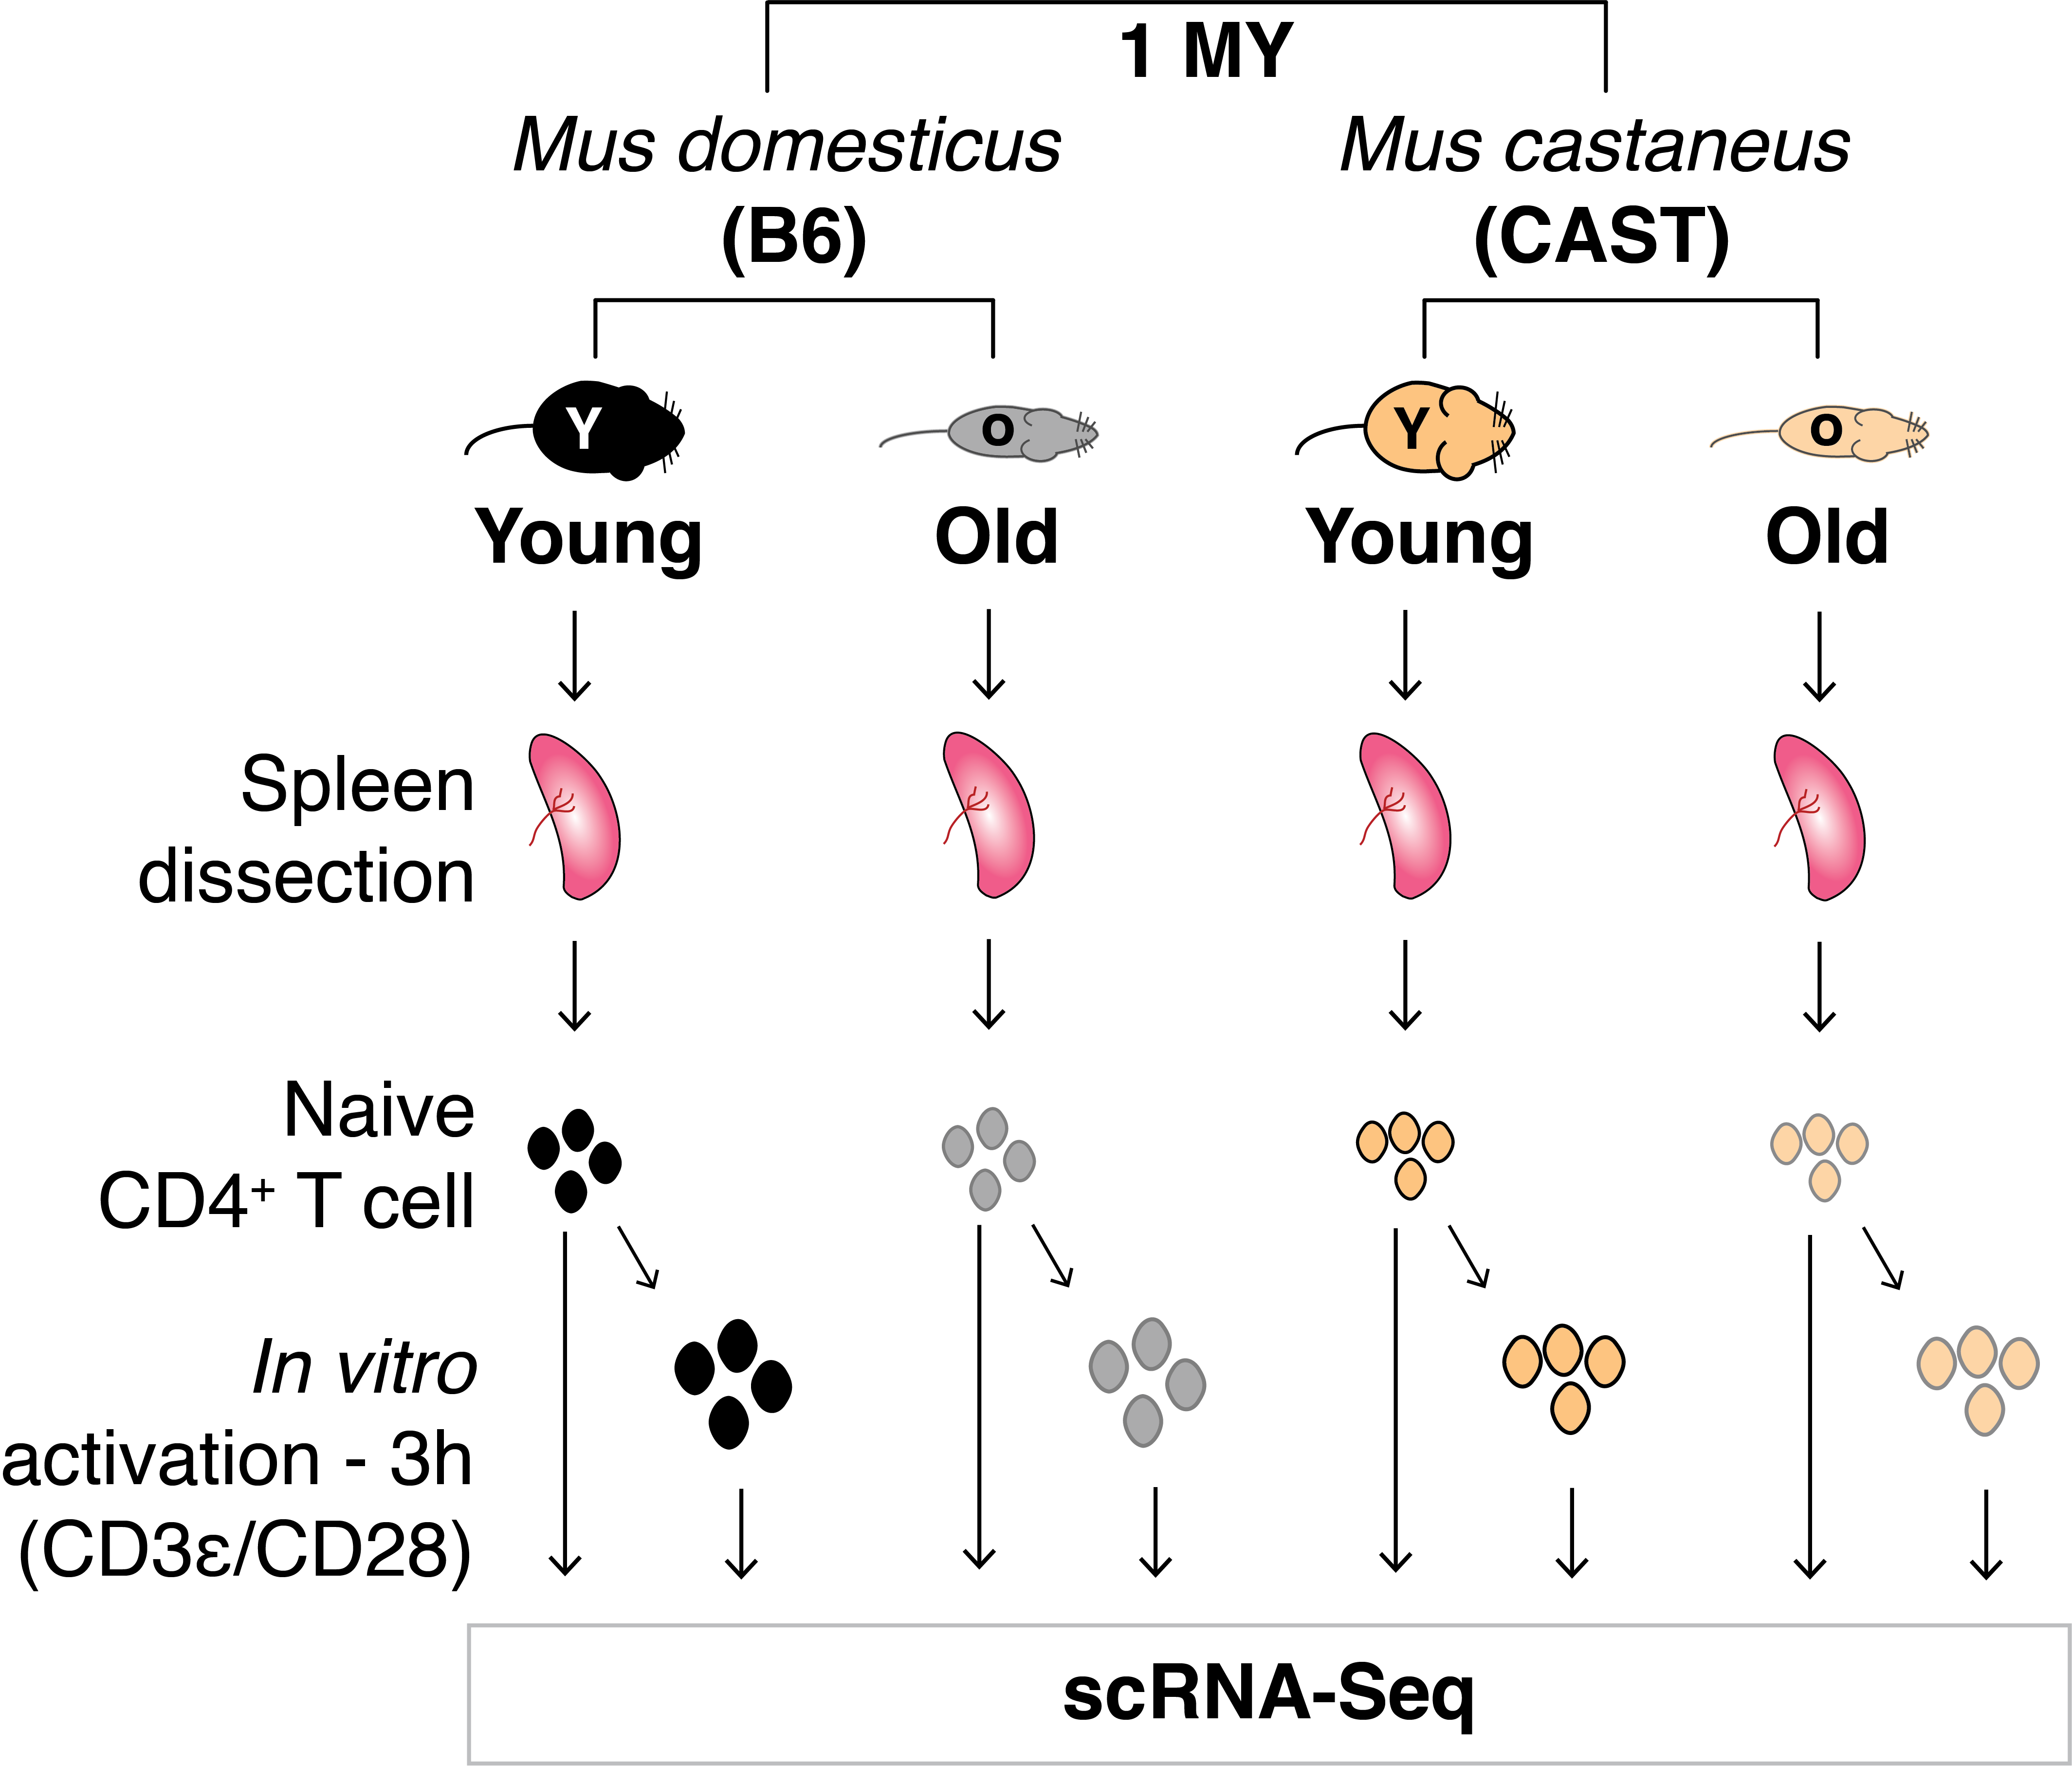
\includegraphics[width=\textwidth]{Fig_1.png}
\caption[Bet-hedging strategy of the \gls{lambdaPhage}]{\textbf{Bet-hedging strategy of the \gls{lambdaPhage}.}\\}
\label{fig0:bedhedging}
\end{figure}

In unicellular organisms, phenotypic heterogeneity facilitates the commitment to alternative cell states in cases of stress (e.g.~nutrient deprivation, temperature fluctuations). For example, \Gls{Bsubtilis} either commits to sporulation or competence upon starvation or DNA damage. Sporulation describes an irreversible process during which vegetative growth ends and the cell forms endospores that survive the altered environment. Competent bacteria on the other hand can take up DNA from these endospores to repair DNA damage \citep{Schultz2009}. The probabilistic and transient activation of competence in a sub-population of \Gls{Bsubtilis} cells is modulated by fluctuations in the competence regulators ComK and ComS. An excitable system of negative and positive feedback loops controls the number of cells that reversibly commit to competence while other cells irreversibly execute sporulation \citep{Suel2006}. Noise in the process of transferring phoshporyl groups across a cascade of regulators maintains a constant probability for cells to commit to sporulation under nutrient deprived conditions \citep{Russell2017}. A similar phenomenon is observed in \Gls{Ecoli} populations exposed to antibiotics where a pre-existing phenotypic heterogeneity allows some cells to resist antibiotic treatment. Once regrown, these cells remain sensitive to the antibiotic \citep{Balaban2004}. \\

Similar to phenotypic heterogeneity in unicellular prokaryotes, transcriptional noise facilitates the switching between mating phenotypes in yeast upon exposure to pheromones \citep{Paliwal2007}. Comparably, commitment to utilizing galactose as nutrient source is a cell fate transition, which is facilitated by stochastic gene expression\cite{Acar2008}. 

\subsection{Development and differentiation}

Similar to bet-hedging strategies in unicellular organisms, noise can facilitate the switch between cell states and the probabilistic induction of differentiation processes \citep{Eldar2010, Chang2008}. It has been shown that transcriptional noise increases throughout differentiation \citep{Stumpf2017} and development \citep{Antolovic2017}. Dissecting differentiation processes of hematopoetic progenitor cells revealed an increase in transcriptional noise directly before cell fate decisions are made \citep{Mojtahedi2016, Richard2016}. Once committed, differentiating cell populations collapse in variability and move towards a new attractor state. This process is aided by variable patterns in DNA methylation states that lock cells in a terminal differentiated state \citep{Jenkinson2017}. \\

Studies of recent years have shown that stochasticity in expression is a crucial driver for early (pre-implantation) embryonic development and prior to gastrulation \citep{Dietrich2007}. As early as the 4-cell stage embryo, targets of master pluripotency markers \Gls{Oct4} and \Gls{Sox2} are heterogeneously expressed.  This is caused by heterogeneous methylation patterns of \Gls{H3R26} induced by \Gls{Carm1}, which in turn facilitates the binding of Oct4 and Sox2 to induce pluripotency. Cell with unmethylated H3R26 differentiate towards the extra-embryonic trophoectoderm while pluripotent cells form the inner cell mass \citep{Goolam2016}. Once the cells compact at the 16-cell stage at \Gls{E} 3.5, cells of the \gls{ICM} stochastically express genes to initiate heterogeneity within the cell population. Fgf4 driven signal reinforcement controls this heterogeneity to form a salt-and-pepper like cell state pattern at E3.5. Positional information and the establishment of gene regulatory networks facilitate the segregation of the epiblast and primitive endoderm lineage \citep{Ohnishi2014}. In line with this, scRNA-Seq revealed high levels of noise in the uncommitted inner cell mass at E3.5 (16-cell stage) in comparison to the E4.5 committed epiblast. Noise levels increase again upon exit from pluripotency in the E6.5 epiblast while cells of the primitive streak at E6.5 synchronize their expression patterns and noise is reduced \citep{Mohammed2017}.

\begin{figure}[!h]
\centering
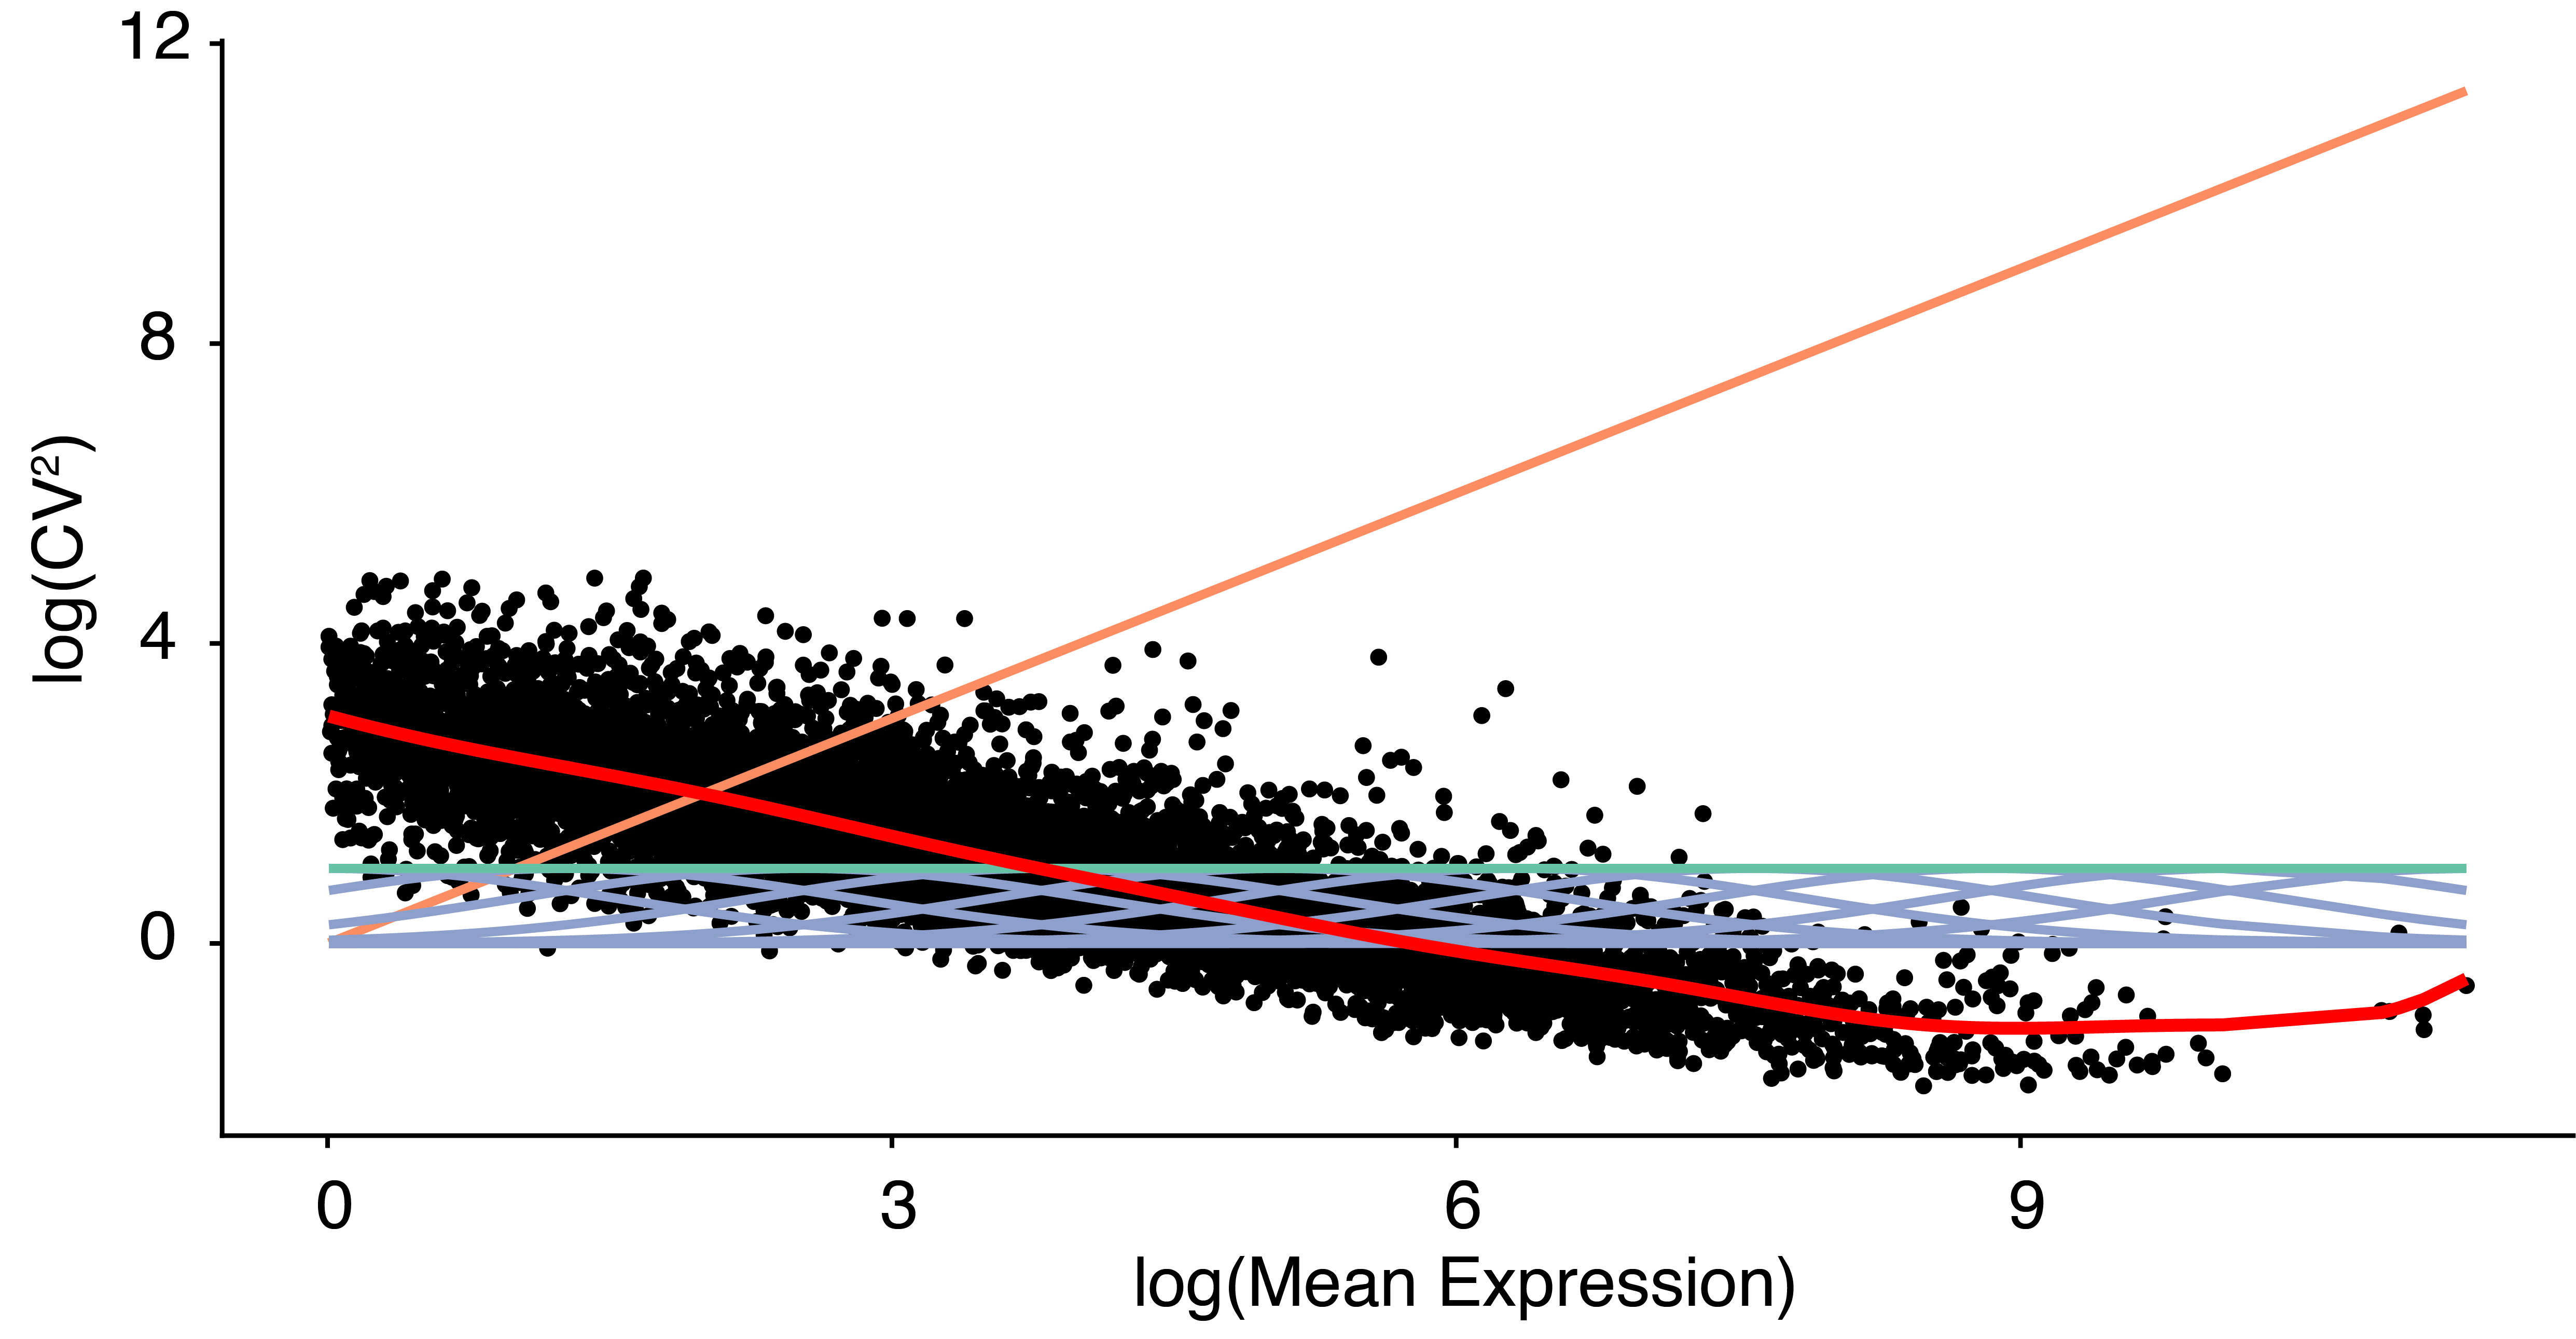
\includegraphics[width=\textwidth]{Fig_2.png}
\caption[Bet-hedging strategy of the \gls{lambdaPhage}]{\textbf{Bet-hedging strategy of the \gls{lambdaPhage}.}\\}
\label{fig0:bedhedging}
\end{figure}

While pluripotent stem cells in the mouse embryo commit irreversibly to cell lineages during development, \emph{in vitro} cultured \glspl{mESC} reside in a self-renewing, metastable state \citep{Hayashi2013}. Heterogenity within the cell population depends on the growth conditions that the cells are being kept in. Transcription factor heterogeneity, especially of the pluripotency regulator Nanog, is highest in \Gls{LIF}/serum grown cells and allows the Nanog-negative cells to commit to differentiation lineages \citep{Chickarmane2012, Torres-Padilla2014}. Heterogeneously expressed genes that show a bimodal distribution in expression counts correlate with each other indicative for the presence of distinct states in mESCs. These distinct states show differences in promoter methylation patterns introducing the role of epigenetic modifications to maintain heterogeneity in mESCs \citep{Singer2014a}. In-depth analysis of mESCs grown in different media (serum, 2i and a2i) shows the presence of three distinct cell states in the serum grown cells. mESCs grown in 2i media show less variability in pluripotency markers but higher heterogeneity in cell-cycle related genes \citep{Kolodziejczyk2015cell}. From the pluripotent ground state, mESCs can differentiate along somatic lineages via specific differentiation events or noise-induced transition between attractor states. Mathematical modelling has shown that mESCs differentiate stochastically through distinct hidden cell (micro-)states within a defined (macro-)state coupled to an increase in variability \cite{Stumpf2017}.\\

In contrast to the beneficial features of noise in stem cell differentiation, stochastic events during \gls{iPSC} reprogramming limit the formation of single iPSCs \citep{Hanna2009, Yamanaka2009}. It has been shown that probabilistic events dominate in an early phase of reprogramming while the transcription of Sox2 induces a later, more deterministic, phase \cite{Buganim2012}. While heterogeneity in gene expression and protein abundance has been characterized to benefit cell commitment and differentiation, other reports propose alternative hypothesis for cell fate decisions where commitment is independent of random fluctuations of transcription factors \cite{Hoppe2016}. Similarly, the increase in noise during development can be counteracted by temporal averaging across noisy transcription events to achieve coordinated tissue responses \citep{Stapel2017}. 

\subsection{Stochasticity in immune responses}

Fast and flexible immune responses are only possible within cell populations that show high plasticity and react to a broad spectrum of stimuli. Stochasticity in cytokine expression leads to phenotypic variability in the \Gls{Th} cell repertoire and increases the effectiveness to respond upon immune stimuli \citep{Schrom2017}. For example, fluctuating expression of lineage defining cytokines \Gls{Ifn}$\gamma$ for Th1 and \Gls{Il} 4 for Th2 in small populations of cells drive the cell population towards a Th1 or Th2 cell fate while most cells co-express the lineage defining transcription factors \Gls{Gata} 3 and \Gls{Tbx21} \citep{Fang2013a, Antebi2013}.\\

Furthermore, Shalek \textit{et al.}, 2014 have shown that upon \Gls{LPS} stimulation a small subset of dendritic cells become activated much earlier than the rest of the cell population while expressing Ifn$\beta$. These early responders support the activation of late responding cells via cell-to-cell communication \citep{Shalek2014}. Likewise, a bimodal (digital) expression of Il2 is detected in T helper cells after immunization where the number of Il2 expressing cells scales with antigen amount. Il2 expressing cells support the activation of surrounding cells via paracrine signaling \citep{Fuhrmann2016}. Similar digital activation processes can be observed in the \Gls{NFkB} signaling pathway. The fraction of cells that activate the this signaling pathway increase with LPS concentration to avoid strong immune activation at low concentrations of a stimulus \citep{Kellogg2015b}.

\begin{figure}[!h]
\centering
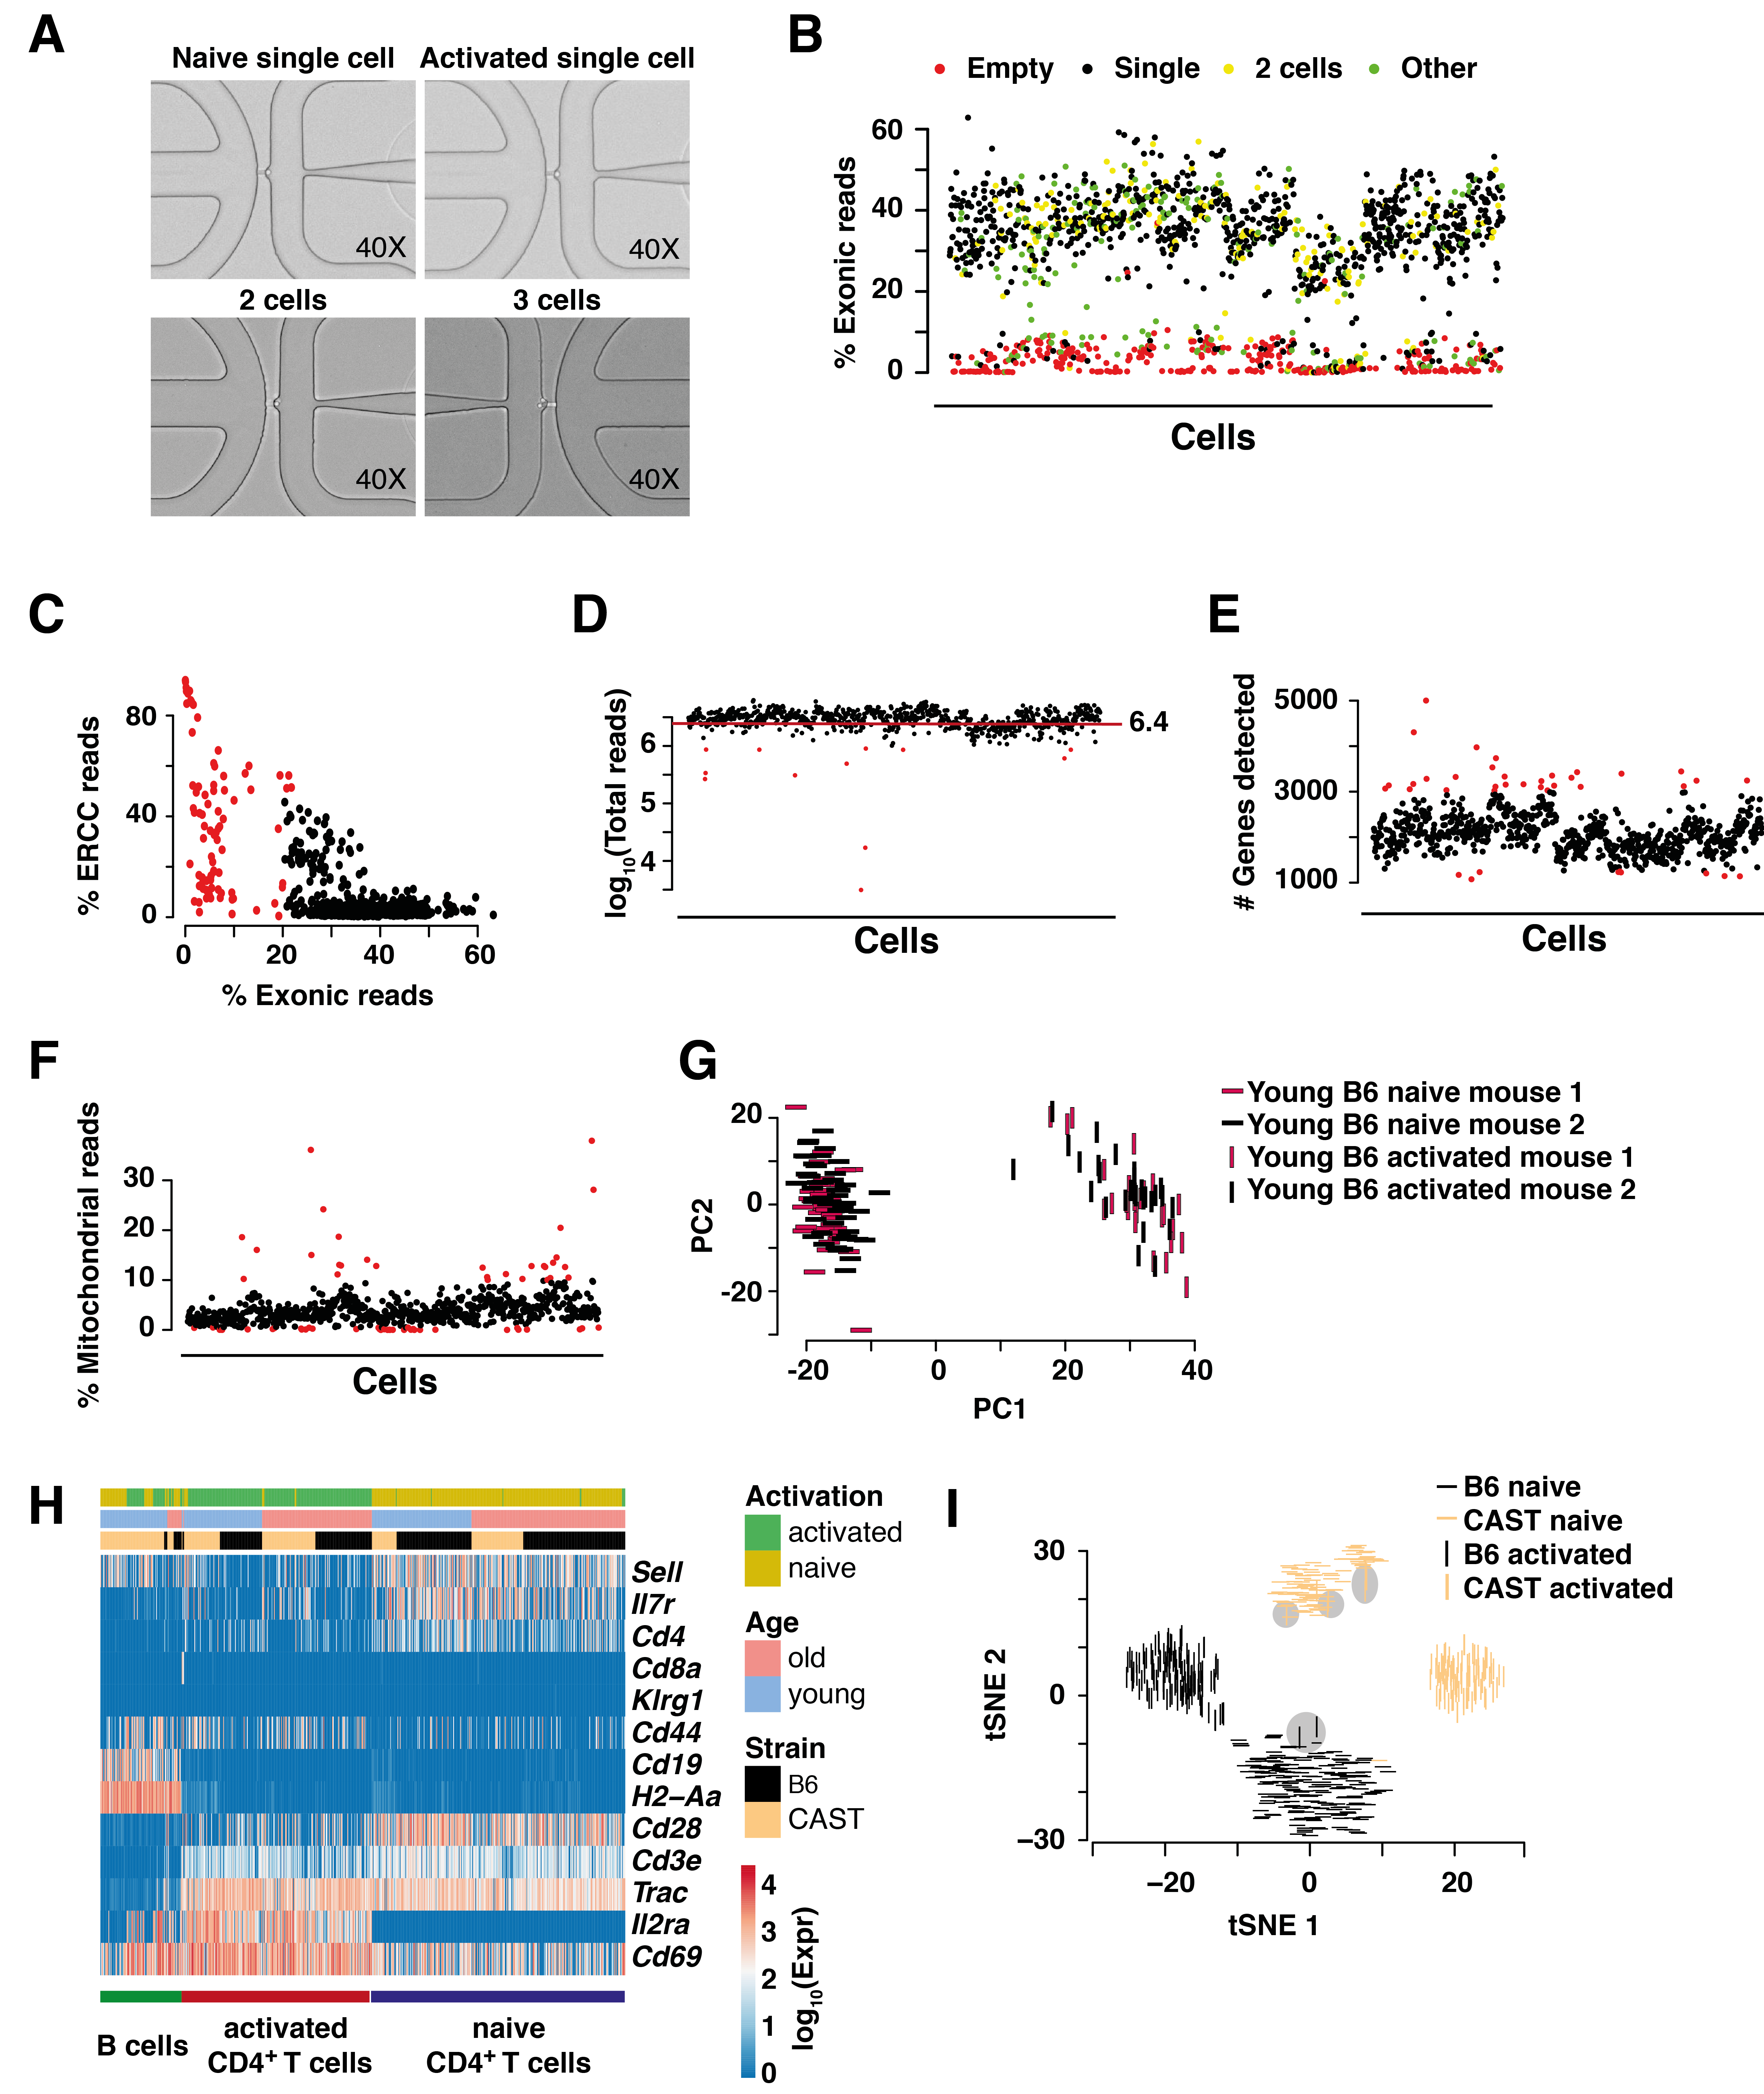
\includegraphics[width=\textwidth]{Fig_3.png}
\caption[Bet-hedging strategy of the \gls{lambdaPhage}]{\textbf{Bet-hedging strategy of the \gls{lambdaPhage}.}\\}
\label{fig0:bedhedging}
\end{figure}

\subsection{Tissue development and homeostasis}

Coping with the influence of biological noise is important for regulated tissue development and homeostasis. An early study showed that in order to minimize the effect of stochasticity in development, plants express heat-shock protein 90 to stabilize metastable regulators of growth and development \citep{Queitsch2002}. Furthermore, redundancy in the \Gls{Celegans} intestinal gene regulatory network buffers variability in the down-stream master regulator \textit{elt-2}. Once highly connected regulators of this network are removed, phenotypic variation arises from bimodal expression of the otherwise highly expressed \textit{elt-2} \citep{Raj2010}. The cooperation of positive and negative feedback loops in these highly connected regulatory networks ensure robust expression of key developmental genes \citep{Ji2013}. While complex signalling networks reduce noise during tissue development, other models have been proposed in which noise helps to form sharp boundaries between neighbouring domains \citep{Zhang2012}. While contact based adhesion and repulsion in between cells sharpens narrow transition regions, noise-driven cell state plasticity helps narrowing a wider transition region \citep{Wang2017}. Conversely, rearrangements within a population of cells, allows the correction of sensing errors induced by variation in the strength of single cell responses to a signalling gradient \citep{Camley2017}.\\

While the cell division rate within tissues is higher during development, tissue homeostasis is maintained by stochastic events that balance cell division and apoptosis \citep{Ranft2010}. The effect of noise on maintaining tissue homeostasis has been studied in a diverse set of organs. In fat tissue, a complex system of signalling feedback loops controls protein abundance noise to induce differentiation at a low rate but prevents stochastic de-differentiation \citep{Ahrends2014}. To maintain coordination in liver function, longer bursts of short lived mRNAs and polyploidy reduce noise in gene expression \citep{BaharHalpern2015}. Another mechanism to achieve tissue-wide expression responses involves spatial coordination of stochastically expressing cells in the pituitary gland \citep{Featherstone2016}. Spatially constraint signalling events have also been demonstrated to play a role in maintaining colonic crypt cell-type diversity. Per crypt, eight stem cells differentiate into a defined ratio of cell-types. To reduce noise in this process, lateral inhibition within a commitment zone reduces the number of differentiated goblet cells and following slower dispersive migration as well as decreased division rates of goblet cells ensures a distinct 1:3 ratio to enterocytes \citep{Toth2017}.

\subsection{Evolution}

As discussed above, biological noise is beneficial for cell fate commitment while in other settings, noise needs to be reduced to allow coordinated expression in cell populations. During evolution, a trade-off between cellular plasticity, the expression responsiveness during environmental changes, and robust expression formed. Natural selection acts on genetically controlled expansions of quantitative phenotypes, which are derived from biological noise \citep{Eldar2010}. For example, noisy expression of stress response genes allows a cell population to adapt to changing environments \citep{Lopez-Maury2009}. Specifically, the expression of genes controlled by TATA-box containing promoters shows strong divergence between species \citep{Tirosh2006}. To control for robust expression levels once selection becomes stabilizing, noise levels are reduced \citep{Lopez-Maury2009, Eldar2010, Pires2016}. \\

Lehner, 2008 discussed specifically evolutionary selection to minimise noise in genes that show harmful phenotypic effects upon alteration ("dosage-sensitive genes"). These genes show low expression noise to reduce the probability of altered expression and also lower expression divergence between species \citep{Lehner2008}. Furthermore, essential genes tend to cluster in the genome in regions with persistent open chromatin to reduce noise \citep{Batada2007}. In line with this, the promoters of core cellular components show a decoupling between expression plasticity and expression noise which indicates that responsiveness in expression is not a general attribute of high expression noise \citep{Lehner2010a}. \\

In unicellular populations, noise evolutionarily increased as a form of rudimentary regulation \citep{Wolf2015}. As a consequence, phenotypic heterogeneity increases the adaption rate of cell populations to extreme environments \cite{Bodi2017}. Conversely, in multicellular organisms, collections of cells need to respond in a coordinated manner. It has therefore been proposed that nuclear compartmentalization in higher organisms reduces noise by mRNA retention at the nuclear membrane \citep{Battich2013, Stoeger2016}.

\subsection{Cancer}

While biological noise supports the adjustment of cells to new microenvironments, errors in the form of gene mutations induce transitions from healthy cells towards a cancer attractor state\citep{Marusyk2012}. Non-genetic heterogeneity aided by transcriptional noise supports the phenotypic adaptation to the new attractor state \citep{Jia2017}. The emergence of non-genetic heterogeneity in tumours is coupled to epigenetic dysregulation that allows the survival of cancer cells \citep{Timp2013}. Furthermore, it has been proposed that genome wide intra-sample methylation heterogeneity is increased in Chronic Lymphoitic Leukemia increasing cancer cell plasticity in the search for new attractor states \citep{Landau2014}.Increased variability in expression can also be observed for more aggressive cancer sub-types across multiple patients \citep{Ecker2015}. \\

An important consequence of biological noise leading to phenotypic heterogeneity in cancer cells is the fractional killing of cell populations upon drug treatment \citep{Flusberg2015}. Noise in proteins mediating \Gls{TRAIL} induced apoptosis leads to the survival of small fractions of cells \citep{Spencer2009}, which could consequently repopulate the tumour environment. Similarly, the stochastic acquisition of DNA damage upon cisplatin exposure introduces heterogeneity in the up-regulation of p53. Slow up-regulation leads to cell-cycle arrest and inhibits apoptosis while only fast up-regulation leads to cell death. In patient derived melanoma cells, sporadic expression of resistance markers forms a rare cell population that grow into resistant colonies after treatment. While pre-resistant cells do not display epigenetic marks and are therefore close to the non-resistant ground state, treatment induces large epigenetic reprogramming forming stable resistant cancer colonies \citep{Shaffer2017}. To tackle this problem, combinatorial therapies have been proposed to reduce variability and fractional killing in cancer cell populations \cite{Paek2016, Roux2015}.

\begin{figure}[!h]
\centering
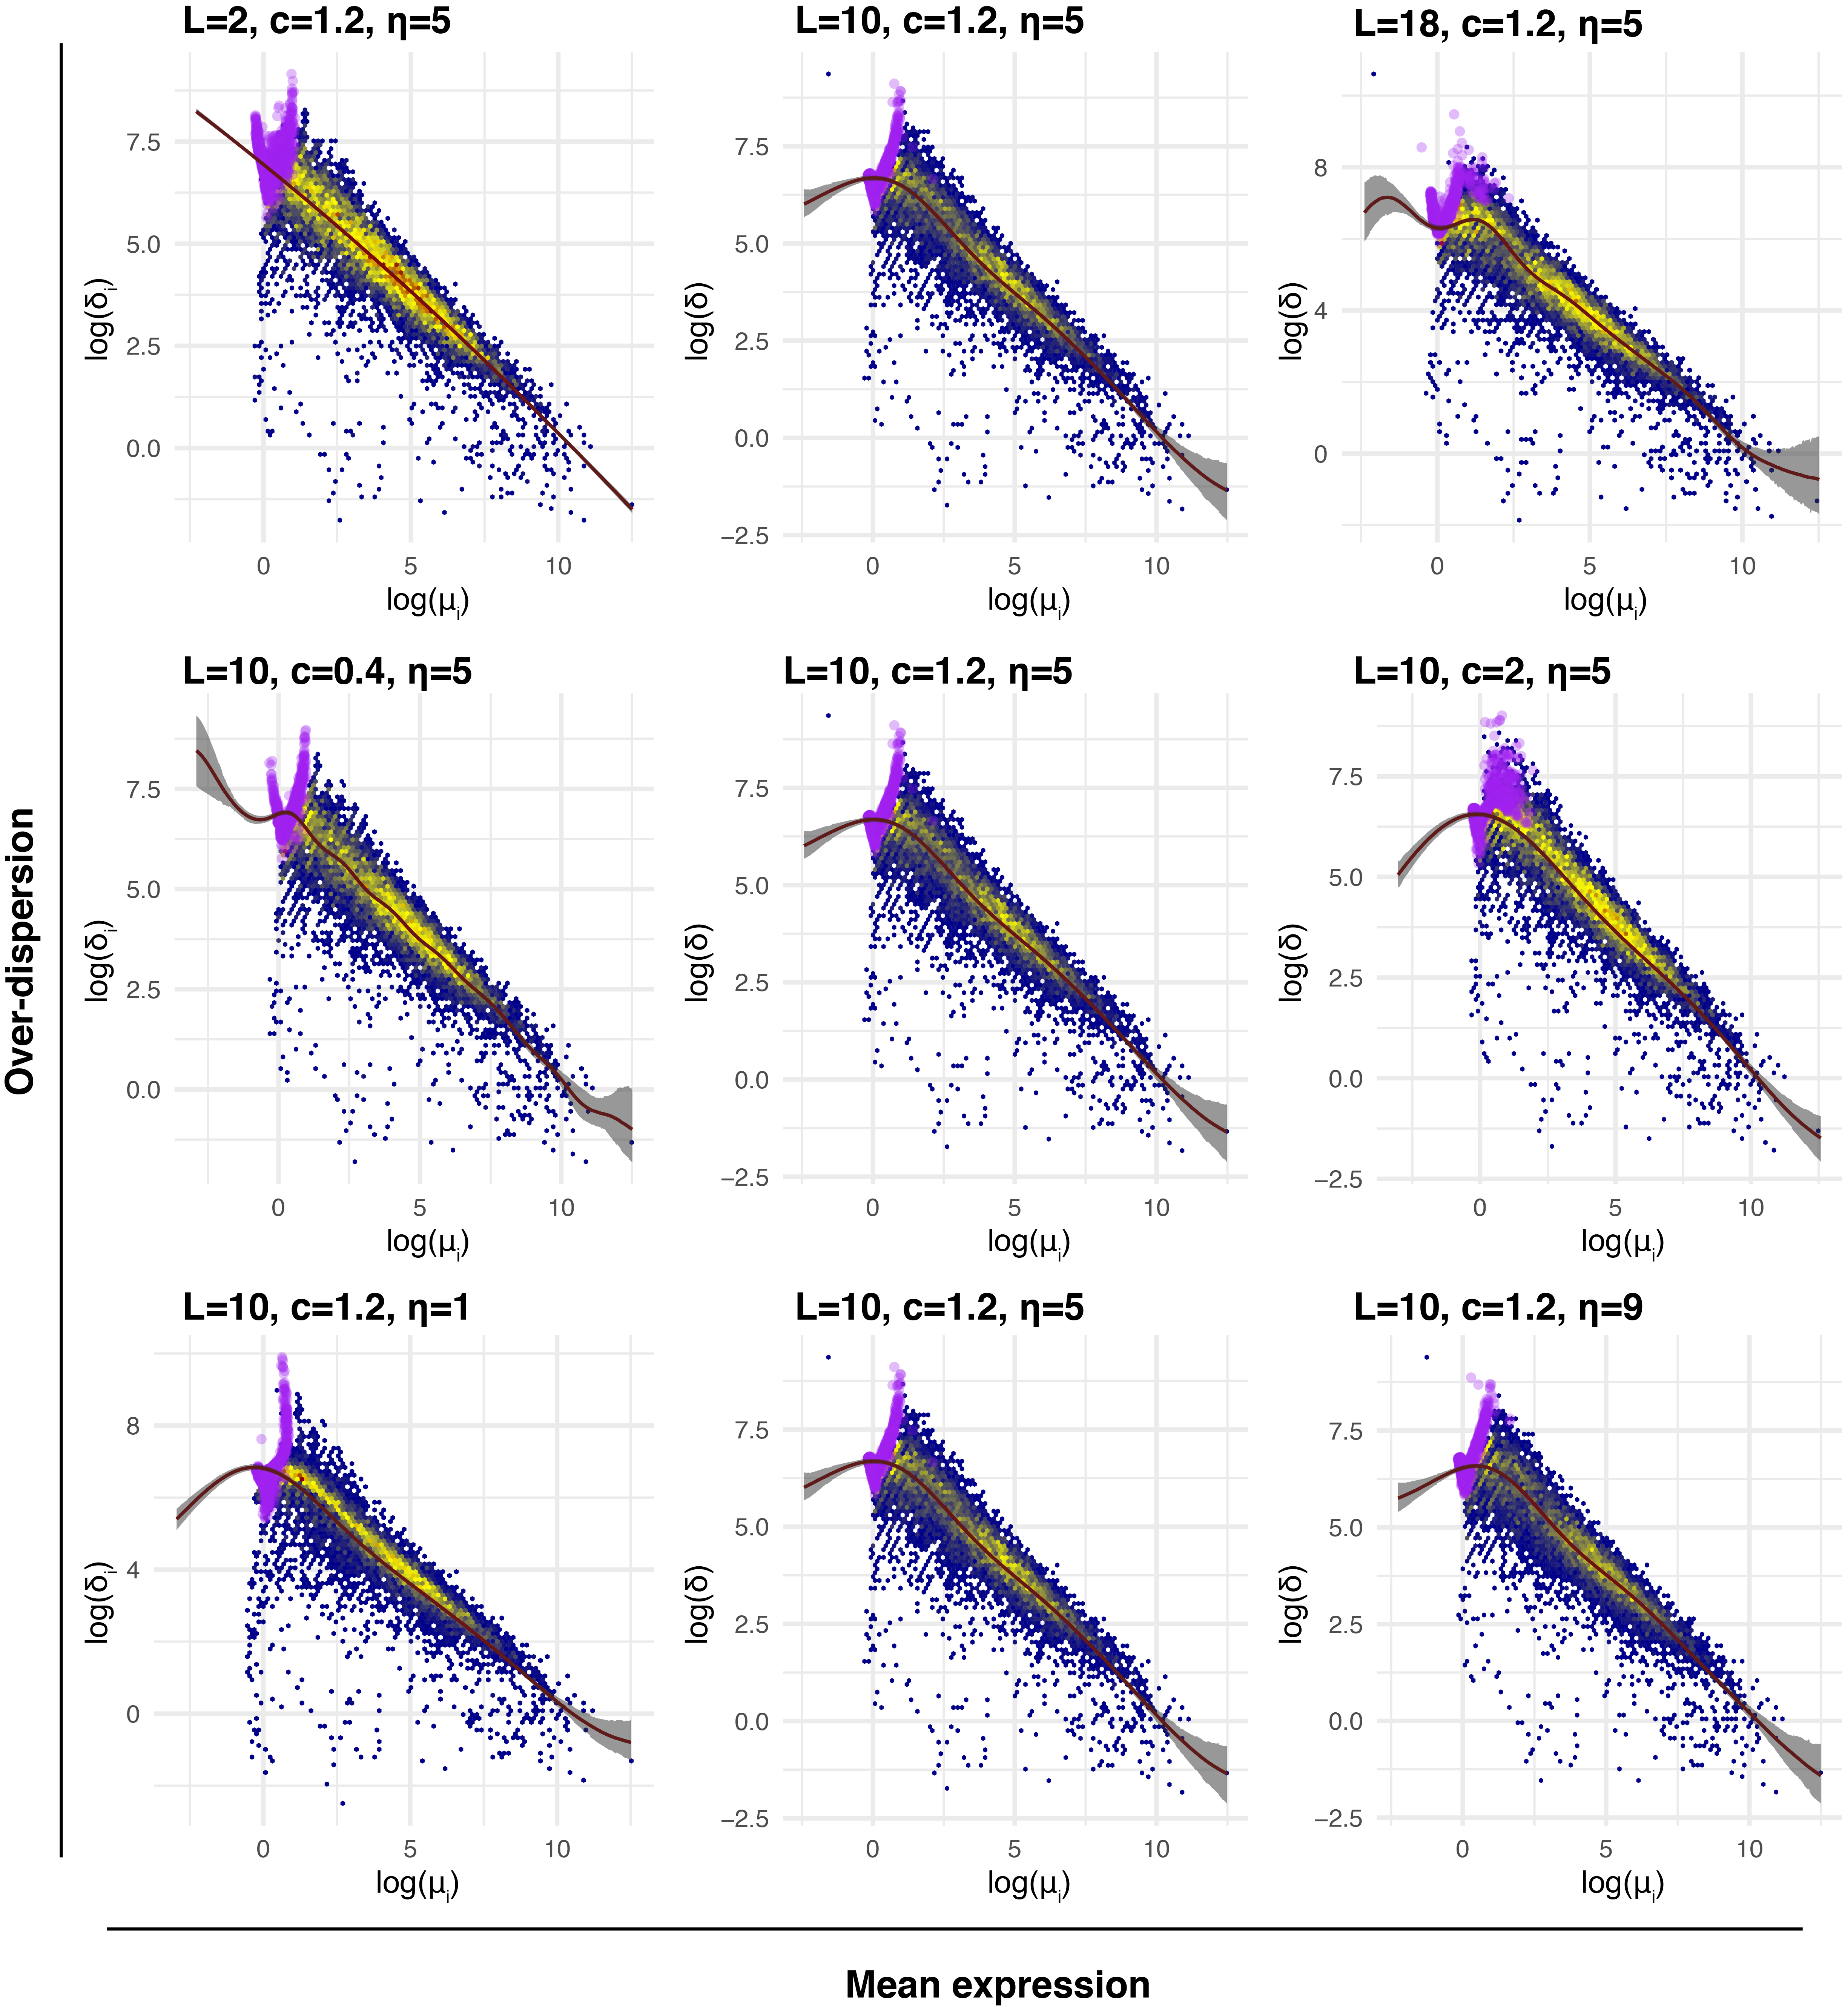
\includegraphics[width=\textwidth]{Fig_4.png}
\caption[Bet-hedging strategy of the \gls{lambdaPhage}]{\textbf{Bet-hedging strategy of the \gls{lambdaPhage}.}\\}
\label{fig0:bedhedging}
\end{figure}

\subsection{Ageing}

Similarly to the onset of cancer, destructive roles of biological noise have been reported during organismal ageing. Previously, it has been debated whether expression noise changes during the lifespan of animals\cite{Bahar2006, Warren2007}. While these initial studies only used small panels of genes, transcriptional profiling of single cells lead to the discovery of a destabilization of the immune activation program in CD4$^+$ T cells due to increased expression noise \cite{Martinez-jimenez2017}. Similarly, transcriptional noise increases with age in human pancreas coupled to an increased stress signature and atypical hormone expression \citep{Enge2017}. 

\newpage

\begin{table}[hb	]
\centering
\caption{Positive and negative effects of biological noise on cellular systems}
\label{table:effects_noise}
\begin{tabular}{l l l}
\toprule
System & Friend & Foe \\ 
\midrule
Unicellular organism & Bet-hedging & \\
\midrule
Development and & Probabilistic induction  & \\
differentiation & of cell differentiation & \\
\midrule
Immune response & Plasticity in immune response & \\
 & Control of response strength &   \\
\midrule
Tissue development  & Low cell differentiation rate & Non-uniform development \\ 
and homeostasis &  & Uncontrolled tissue response \\
\midrule
Evolution & Adjustment to  & Non-uniform, stabilizing expression \\ 
& fluctuating environment & Uncontrolled tissue responses \\
\midrule
Cancer &  & Phenotypic adaption to cancer state \\
& & Fractional killing of cancer cells \\
\midrule
Aging &  & Unsynchronized immune response \\
& & Increased stress signatures \\ 
\bottomrule
\end{tabular}
\end{table}
